\documentclass{report}

\usepackage{graphicx}
\usepackage{titlesec}
\usepackage{siunitx}
\usepackage[margin=1in]{geometry}
\usepackage{lscape}
\usepackage{rotating}
\usepackage{subcaption}
\usepackage{pdfpages}
\usepackage{changepage}
\usepackage{wrapfig}
\usepackage{hyperref}
\usepackage{listings}
\lstset{
	basicstyle=\small\ttfamily,
	columns=flexible,
	breaklines=true
}
\newcommand\tab[1][1cm]{\hspace*{#1}}


%This forces tables and figures placed in a section to stay
% in that section rather than floating away
\usepackage[section]{placeins}


%This suppresses each chapter displaying "Chapter X"
%\titleformat{\chapter}[display]
%{\normalfont\bfseries}{}{0pt}{\Large}

%This handles the formatting of chapter headings
% {left spacing}{before spacing}{after spacing}
\titlespacing*{\chapter}{0pt}{0pt}{0pt}

%This handles the formatting of section headings
% {left spacing}{before spacing}{after spacing}
\titlespacing*{\section}{0pt}{10pt}{0pt}

%This handles the formatting of subsection headings
% {left spacing}{before spacing}{after spacing}
\titlespacing*{\subsection}{0pt}{0pt}{5pt}

%This handles the formatting of subsubsection headings
% {left spacing}{before spacing}{after spacing}
\titlespacing*{\subsubsection}{0pt}{5pt}{0pt}


%Set up chapter
\title
{
	\textbf{{ROS-Gazebo-ErleRover Installation and Usage Guide}\\
	{Michigan State University}\\
	{ECE 480}\\}
	
\includegraphics{Images/MSU_Lab_Cover_Image.png}
}

\author{Glen Simon\\
Philip McKinley\\
Jared Moore\\
Anthony Clark}


%Current date will auto add here

\begin{document}
\maketitle

\newpage
%To update table of contents have to edit the line then build
\tableofcontents
\clearpage

\chapter{Introduction}

\chapter{Installation}
These installation directions are derived from the instructions provided by Erle Robotics found at\\ \href{http://docs.erlerobotics.com/simulation/configuring\_your\_environment}{http://docs.erlerobotics.com/simulation/configuring\_your\_environment}.
\\

It is recommend that this software is used on a machine running Ubuntu 14.04 64 bits.

\section{Configuring your Ubuntu Machine}
These steps only have to be done once per machine.
\subsection{Install base packages}
\begin{lstlisting}
	sudo apt-get update
	sudo apt-get install gawk make git curl cmake -y
\end{lstlisting}

\subsection{Install dependencies for MAVProxy}
\begin{lstlisting}
	sudo apt-get install g++ python-pip python-matplotlib python-serial python-wxgtk2.8 python-scipy -y
	sudo apt-get install python-opencv python-numpy python-pyparsing ccache realpath libopencv-dev -y
\end{lstlisting}

\subsection{Install MAVProxy}
\begin{lstlisting}
	sudo pip install future
	sudo apt-get install libxml2-dev libxslt1-dev -y
	sudo pip2 install pymavlink catkin_pkg --upgrade
	sudo pip install -I MAVProxy==1.5.2
\end{lstlisting}

\subsection{Download and install ArUco}
\begin{enumerate}
	\item Download ArUco 1.3.0 from here \href{https://sourceforge.net/projects/aruco/files/1.3.0/aruco-1.3.0.tgz/download}{https://sourceforge.net/projects/aruco/files/1.3.0/aruco-1.3.0.tgz/download}
	
	\item Install ArUco

\begin{lstlisting}
	cd ~/Downloads # Replace this with your Download directory
	tar -xvzf aruco-1.3.0.tgz
	cd aruco-1.3.0/
	mkdir build && cd build
	cmake ..
	make
	sudo make install
\end{lstlisting}
\end{enumerate}

\subsection{Install ROS Indigo}
\subsubsection{Setup your computer to accept software from packages.ros.org, setup your keys and install (make sure your Debian package index is up-to-date):}
\begin{lstlisting}
	sudo sh -c 'echo "deb http://packages.ros.org/ros/ubuntu $(lsb_release -sc) main" > /etc/apt/sources.list.d/ros-latest.list'
	sudo apt-key adv --keyserver hkp://ha.pool.sks-keyservers.net --recv-key 0xB01FA116
	sudo apt-get update
\end{lstlisting}

\subsubsection{Install, ROS package, build, and communication libraries. No GUI tools.:}
\begin{lstlisting}
	sudo apt-get install ros-indigo-ros-base -y
\end{lstlisting}

\subsubsection{Initialize rosdep, before you can use ROS, you will need to initialize rosdep. rosdep enables you to easily install system dependencies for source you want to compile and is required to run some core components in ROS.}
\begin{lstlisting}
	sudo rosdep init
	rosdep update
\end{lstlisting}

\subsubsection{It's convenient if the ROS environment variables are automatically added to your bash session every time a new shell is launched:}
\begin{lstlisting}
	echo "source /opt/ros/indigo/setup.bash" >> ~/.bashrc
	source ~/.bashrc
\end{lstlisting}

\subsubsection{Get rosinstall and some additional dependencies}
\begin{lstlisting}
	sudo apt-get    install python-rosinstall          \
	ros-indigo-octomap-msgs    \
	ros-indigo-joy             \
	ros-indigo-geodesy         \
	ros-indigo-octomap-ros     \
	ros-indigo-mavlink         \
	ros-indigo-control-toolbox \
	ros-indigo-transmission-interface \
	ros-indigo-joint-limits-interface \
	unzip -y
\end{lstlisting}

\subsubsection{Get RQT graph}
\begin{lstlisting}
sudo apt-get install ros-indigo-rqt
sudo apt-get install ros-indigo-rqt-common-plugins
\end{lstlisting}


\subsection{Install Gazebo}
\subsubsection{Setup your computer to accept software from packages.osrfoundation.org}
\begin{lstlisting}
	sudo sh -c 'echo "deb http://packages.osrfoundation.org/gazebo/ubuntu-stable `lsb_release -cs` main" > /etc/apt/sources.list.d/gazebo-stable.list'
\end{lstlisting}

\subsubsection{Setup keys}
\begin{lstlisting}
	wget http://packages.osrfoundation.org/gazebo.key -O - | sudo apt-key add -
\end{lstlisting}

\subsubsection{Install gazebo7}
\begin{lstlisting}
	sudo apt-get update
	sudo apt-get remove .*gazebo.* '.*sdformat.*' '.*ignition-math.*' && sudo apt-get update && sudo apt-get install gazebo7 libgazebo7-dev drcsim7 -y
\end{lstlisting}


\chapter{Configuring User Workspace}
These steps will have to be done for each user on a machine if they would like their own local copies of the source files.

\section{Download Ardupilot}
The ArduPilot project is an open source autopilot for drones. We'll be using its code to simulate the UAVs:
\subsection{Compile a specific branch of ardupilot}
\begin{lstlisting}
	mkdir -p ~/simulation; cd ~/simulation
	git clone https://github.com/erlerobot/ardupilot -b gazebo
\end{lstlisting}

\section{Download ErleRover\_Scripts directory}
This was created to ease the process of starting all of the required processes used to simulate the Erle Rover.
\begin{lstlisting}
	cd ~/simulation
	git clone https://github.com/gsimon2/ErleRover-Scripts.git
\end{lstlisting}
\subsection{Getting permission to push commits to the remote repo}
This is a public repo and can freely be copied, but for access to submit changes please contact Glen Simon at glen.a.simon@gmail.com.

\section{Download ros\_gazebo\_python directory, which contains the BasicBot work. Optional}
\begin{lstlisting}
	cd ~/simulation
	git clone https://github.com/jaredmoore/ros_gazebo_python.git
\end{lstlisting}
\subsection{Getting permission to push commits to the remote repo}
This is a public repo and can freely be copied, but for access to submit changes please contact Jared Moore at swiftfoottim@gmail.com.



\section{Create ROS workspace}
\subsection{Make workspace}
\begin{lstlisting}
	mkdir -p ~/simulation/ros_catkin_ws/src
\end{lstlisting}

\subsection{Initialize the workspace}
\begin{lstlisting}
	cd ~/simulation/ros_catkin_ws/src
	catkin_init_workspace
	cd ~/simulation/ros_catkin_ws
	catkin_make
	source devel/setup.bash
\end{lstlisting}

\subsection{Download ros\_catkin\_ws\_src which contains the development work for the MSU rover project}
\begin{lstlisting}
	cd ~/simulation/ros_catkin_ws
	git clone https://github.com/gsimon2/ros_catkin_ws_src.git
\end{lstlisting}

\subsubsection{Delete default src directory and replace with the downloaded one}
\begin{lstlisting}
	cd ~/simulation/ros_catkin_ws
	rm -r src
	mv ros_catkin_ws_src src
\end{lstlisting}

\subsubsection{Getting permission to push commits to the remote repo}
This is a public repo and can freely be copied, but for access to submit changes please contact Glen Simon at glen.a.simon@gmail.com.

\subsection{Compile the ros\_catkin\_ws workspace}
\begin{lstlisting}
	cd ~/simulation/ros_catkin_ws
	source devel/setup.bash
	catkin_make --pkg mav_msgs mavros_msgs gazebo_msgs
	catkin_make -j 4
\end{lstlisting}

\section{Download Gazebo models}
\begin{lstlisting}
	mkdir -p ~/.gazebo/models
	git clone https://github.com/erlerobot/erle_gazebo_models
	mv erle_gazebo_models/* ~/.gazebo/models
\end{lstlisting}

\section{Configuring .bashrc}
\subsection{Add ROS setup to bash}
	It's convenient if the ROS environment variables are automatically added to your bash session every time a new shell is launched.
\begin{lstlisting}
	echo "source /opt/ros/indigo/setup.bash" >> ~/.bashrc
	source ~/.bashrc
\end{lstlisting}

\subsection{Add ros\_catkin\_ws setup to bash}
	For ROS to find the packages provided in ros\_catkin\_ws we need to source the setup file every time. This is easier if we also add this to the bash file.
\begin{lstlisting}
	echo "source ~/simulation/ros_catkin_ws/devel/setup.bash" >> ~/.bashrc
	source ~/.bashrc
\end{lstlisting}


\chapter{Usage}
\section{Basic Erle-Rover simulation}
This process will bring up the Erle-Rover in a blank world and allow you to manually enter throttle and yaw commands via the MAVProxy terminal.
\subsection{Manually starting all needed processes}
The process of starting all processes can be found in more detail at: \\ \href{http://docs.erlerobotics.com/simulation/vehicles/erle_rover/tutorial_1}{http://docs.erlerobotics.com/simulation/vehicles/erle\_rover/tutorial\_1}, but will be covered briefly here.
\subsubsection{Executing APMrover2}
This process requires two active terminals. 

In terminal one enter:
\begin{lstlisting}
	source ~/simulation/ros_catkin_ws/devel/setup.bash
	cd ~/simulation/ardupilot/APMrover2
	../Tools/autotest/sim_vehicle.sh -j 4 -f Gazebo
	# once MAVProxy has launched completely, load the parameters
	param load /[path_to_your_home_directory]/simulation/ardupilot/Tools/Frame_params/3DR_Rover.param
	# NOTE: replace [path_to_your_home_directory] with the actual path to your home directory.
	# Example: param load /home/john/simulation/ardupilot/Tools/Frame_params/3DR_Rover.param
\end{lstlisting}

In terminal two enter:
\begin{lstlisting}
	source ~/simulation/ros_catkin_ws/devel/setup.bash
	roslaunch ardupilot_sitl_gazebo_plugin rover_spawn.launch
\end{lstlisting}

This should start the Gazebo GUI and you should be able to see that the rover spawned in a blank world appearing similar to figure \ref{Erle-Rover-model}.

\begin{figure}[ht]
	\centering
	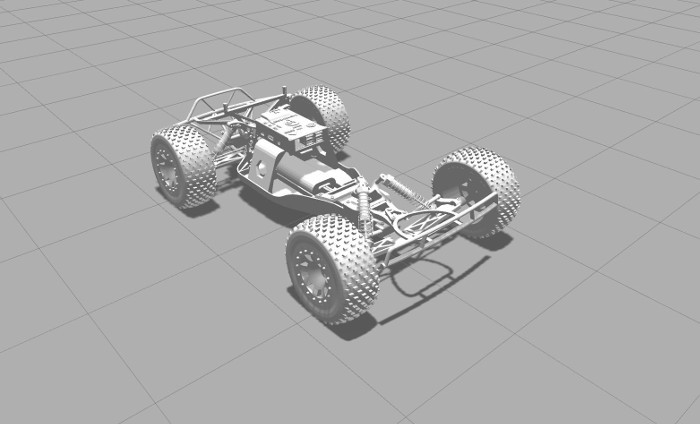
\includegraphics[scale = 0.35]{Images/rover}
	\caption{Erle-Rover model in Gazebo simulator}
	\label{Erle-Rover-model}
\end{figure}

\subsubsection{Controlling Erle-Rover using MAVProxy}
Make the rover move forward. In the first terminal execute:
\begin{lstlisting}
	# in the MAVProxy prompt:
	mode MANUAL
	param set SYSID_MYGCS 255
	rc 3 1900
\end{lstlisting}
Or backwards:
\begin{lstlisting}
	# in the MAVProxy prompt:
	rc 3 1200
\end{lstlisting}
What we are doing here is override the 3rd channel of the RC, which corresponds to the throttle. Values go from 1100 to 1900. 1500 is to stop the throttle; so values above 1500 will make the rover move forward, and values above 1500 backwards. The same principle applies to the yaw, which is in the 1st channel of the RC. Values above 1500 will make it turn right, and below 1500 left. For instance:
\begin{lstlisting}
	# in the MAVProxy prompt:
	rc 1 1400
\end{lstlisting}

\subsection{Using scripts to start simulation}


\section{Basic obstacle avoidance simulation}

\section{Line follower simulation}

\section{Object finder simulation}






\end{document}
